\documentclass[12pt, handout]{beamer}
\usepackage[polytechnique, psc, complexe, unicouleur]{persobeamer}
%nocouleur ou: unicouleur ou~: bicouleur
%complexe ou~: simple
%voir dans le package pour changer les couleurs
\usepackage{tikz}

\title{Projet Scientifique collectif INF02}
\subtitle{Soutenance finale}
\author{}
\date{19 mai 2015}

%%change to "<hide notes"> if you want
%% avec show notes, le logo plante, c'est normal
\setbeameroption{show notes}

\begin{document}

  \addtobeamertemplate{frametitle}{}{%
    \begin{tikzpicture}[remember picture,overlay]
    \node[anchor=south east,yshift=2pt] at (current page.south east) {
\includegraphics[height=0.7cm]{./images/logohori.jpg}};

    \end{tikzpicture}
   }

    \begin{frame}
      \maketitle
    \end{frame}		


    %% sommaire %%		
    \begin{frame}
      \frametitle{Sommaire}
      %\tableofcontents[pausesections]
      \tableofcontents
    \end{frame}

%%%%%%%%%%%%%%%%%%%%%%%%
\section{Introduction}
%%%%%%%%%%%%%%%%%%%%%%%%%%

%%%%%%%%%%%%%%%%
\begin{frame}
 \frametitle{But du projet}
 
 \begin{block}{Résumer un texte}
   \begin{itemize}
  \item Étant donné un article sportif ;
  \item En donner les idées majeures.
 \end{itemize}
 \end{block}

 Travail sur des données pré-traitées sur le plan grammatical.

 \note{ Notre but était de produire un programme qui, étant donné un article sportif (de foot), serait capable d'en donner l'idée principale.
 
 La complexité de l'analyse syntaxique nous a amené à travailler sur des données pré-traitées contenant déjà l'information grammaticale du texte.}
 
\end{frame}

%%%%%%%%%%%%%%%%%%%
\begin{frame}
 \frametitle{Modules}
 
 \begin{itemize}
  \item Construction d'un Réseau de Concepts~;
  \item Traitement des données grammaticales~;
  \item Construction d'un Workspace~;
  \item Algorithme de résumé statistique~;
  \item Algorithme de résumé abstractif.
 \end{itemize}
 
 \note{Nous avons pu séparer le travail en plusieurs modules relativement indépendants.}
 
\end{frame}


\begin{frame}
 \frametitle{Organisation générale}
 %% qui a fait quoi, comment, quand etc...
 
\end{frame}

\begin{frame}
 \frametitle{Outils extérieurs et points techniques}
 %% Je serais d'avis d'éliminer cette slide (Antonin)
 %% pareil (andré)
 
\end{frame}

%%%%%%%%%%%%%%%%%%%%%%%%%%%%%%
\subsection{État de l'art}
%%%%%%%%%%%%%%%%%%%%%%%%%%%%%

%%%%%%%%%%%%%%%%%%%%
\begin{frame}
 \frametitle{Traitement du langage naturel}
 Des outils existent déjà pour~:
 \begin{itemize}
  \item Reconnaître des mots, synonymes, etc. (\texttt{nltk}, \texttt{WordNet})
  \item Établir la structure grammaticale d'une phrase (\texttt{nltk}, \texttt{Systran})
 \end{itemize}
 Nous voulions utiliser ces outils pour résumer des textes.
 
\end{frame}

%%%%%%%%%%%%%%%%%%%%%ù
\begin{frame}
 \frametitle{\textit{Extractive summarization}}
%% Un algorithme de résumé extractif~:
 \begin{itemize}
  \item Sépare les phrases du texte~;
  \item Note ces phrases d'après une étude statistique~;
  \item Sélectionne les phrases les mieux notées et les copie dans le résumé.
 \end{itemize}
 
\end{frame}

%%%%%%%%%%%%%%%%%%%%%%%
\begin{frame}
 \frametitle{\textit{Abstractive summarization}}
 %%Un algorithme de résumé abstractif tentera d'étudier les informations du texte~:
 \begin{itemize}
  \item Représentation du texte en mémoire sous forme d'un arbre syntaxique~;
  \item Élagage de cet arbre pour ne garder que les nœuds importants~;
  \item Génération d'un texte en langage naturel à partir de l'arbre simplifié.
 \end{itemize}
 \note{On remarque que la première et la dernière étape sont beaucoup plus difficiles que leurs analogues en résumé extractif.}
\end{frame}


% \begin{frame}
%  \frametitle{Génération du résumé et évaluation}
%  %% D'avis de virer ça (Antonin)
%  %% pareil, même si ça me rend triste (andré)
%  
% \end{frame}

%%%%%%%%%%%%%%%%%%%%%%%%%%%%%%
\section{Sources de données}
%%%%%%%%%%%%%%%%%%%%%%%%%%%%%%%%%%ù

%\subsection{Données textuelles}

\begin{frame}
 \frametitle{Données textuelles}
 \begin{itemize}
  \item Sélection d'un certain nombre de flux RSS pour téléchargement automatique d'articles~;
  \item Pré-traitement par une API (readability) pour n'obtenir que le corps de l'article.
 \end{itemize}
 
 \note{Notes à compléter ?}
 
\end{frame}

%\subsection{Données conceptuelles}

%%%%%%%%%%%%%%%%%%%%%%%%%%%%%
\begin{frame}
 \frametitle{Extraction de concepts}

 \begin{itemize}
  \item Mise sous forme normale (WordNet) ;
  \item \textit{POS-tagger} ;
  \item Sélection des noms propres.
 \end{itemize}
 
 \note{Du texte brut, on peut extraire les concepts en un certain nombre d'étapes. Pour ça on se sert de wordnet interfacé avec nltk, et de toutes ses infos grammaticales, avec morphy qui "morphe" les mots, ie les met sous forme normale directement. Le POS-taggers de nltk est utile car l'envoi d'une info supplémentaire de pos à morphy permet de limiter d'autant plus le nombre d'erreurs. Enfin, ça permet aussi de sélectionner les noms propres dont le traitement doit se faire à part.}
 
\end{frame}

%%%%%%%%%%%%%%%%%%%%%%%%
\begin{frame}
 \frametitle{Données conceptuelles}
 
 \begin{block}{Conceptnet5}
   Graphe sémantique porteur de nombreuses relations. %(RelatedTo, IsA...)
    
  Requêtes :
  \begin{itemize}
    \item LookUp ;
    \item Search ;
    \item Association.
  \end{itemize}

  On sélectionne les concepts les plus pertinents.
 \end{block}

 \pause
 
\begin{block}{Freebase}
 Traitement des noms propres.
\end{block}

 \note{Conceptnet5 appartient au Commonsense computing initiative, généré à partir de données brutes.
 1,6 millions d'assertions. On récupère une partie des concepts, une partie des assertions (on évite certaines relations trop floues comme RelatedTo). Freebase : permet de traiter les noms propres, on n'a pas utilisé toutes les possibilités offertes par l'API mais déjà ça c'était utile.}
\end{frame}


%%%%%%%%%%%%%%%%%%%%%%%%%%%
\section{Réseau de concepts}
%%%%%%%%%%%%%%%%%%%%%%%%%%%
% Schrotty !

\subsection{Structure}

\begin{frame}
 \frametitle{Objectifs et utilité du réseau}
 
 \begin{itemize}
  \item Représenter des données conceptuelles~;
  \item Établir des relations sémantiques~;
  \item Fournir des informations de contexte.
 \end{itemize}
 
 Le réseau sert à \textbf{sélectionner} de l'information.
 \note{Initialement le RC naît de la nécessité d'ajouter de l'info de type contexte lorsqu'on lit le texte. Ses prérogatives ont évolué au cours du projet ; finalement il s'est convenablement marié au workspace que l'on verra plus tard. Son caractère dynamique est resté essentiel même s'il a lui aussi évolué. -----------
 Explication : plus loin on verra que les noeuds du RC activés, propagent, et on supprime dans le Workspace les concepts les moins activés.} 
\end{frame}

%%%%%%%%%%%%%%%%
\begin{frame}
 \frametitle{Structure du réseau}
 
 \begin{block}{N\oe{}uds}
    \begin{itemize}
      \item Étiquette~: concept~;
      \item Importance conceptuelle~;
      \item Activation~;
    \end{itemize}
   \textbf{Exemple~:} [``hyperactivity'', ``ic'': 34, ``a'': 10].
\end{block}

  \begin{block}{Arêtes}
    \begin{itemize}
      \item Orientées~;
      \item Proximité~;
      \item Relation.
    \end{itemize}
    \textbf{Exemple~:} [``hyperactivity'', ``disorder'', \{``r'': ``IsA'', ``w'': 47\}]. 
  \end{block}

\note{RC - réseau sémantique, les noeuds ont quelques informations qui s'interprètent facilement, un mot, une importance conceptuelle dont il faudra parler plus tard mais qui rep. juste le degré d'abstraction et d'importance du concept : pour nous, lié au foot implique très important, matériel implique moins important. Ici ça a son importance, mais c'est peu important dans notre contexte, donc ic assez bas.}

  \note{---------------------------- Les relations, sur le modèle de conceptnet5, et tout aussi proches de l'intuition. Représentent une connaissance. Le poids est une proximité, à quel point il est facile de penser à un concept en partant d'un autre.}

\end{frame}


%%%%%%%%%%%%%%%%%%%%%%%%%%%%%%%%%%%%%%%
\begin{frame}[fragile]
 \frametitle{Propriétés dynamiques du réseau}
 
 \begin{itemize}
  \item L'activation d'un n\oe{}ud se propage à ses fils~;
  \item Les n\oe{}uds se désactivent naturellement.
 \end{itemize}
 
 \textbf{Exemple 1~:} en partant de \verb|``wayne_rooney''| et  \verb|``manchester_united_f.c.''|.
 
 \textbf{Exemple 2~:} en considérant les n\oe{}uds fortement activés (plus de 10\%).
 
 \note{ Sur le premier exemple, on ne montre pas le degré d'activation de chaque noeud, c'est juste pour voir la propagation. Sur le deuxième on s'intéresse déjà plus à la pertinence.}
 
\end{frame}


%%%%%%%%%%%%%%%%%%%%%%%%%%%%%%%
\begin{frame}
  \frametitle{Exemple 1}
  
  \begin{itemize}
 \item Étape 0~: 2  n\oe{}uds activés.
 \item Étape 1~: 6  n\oe{}uds activés.
 \item Étape 2~: 67 n\oe{}uds activés.
  \end{itemize}

  \note{Envoyer ici l'exemple touslesnoeuds sur une autre fenêtre. Ce sont wayne rooney et manchester activés tous les deux en même temps à 60\%. On remarque que le nombre de noeuds touchés augmente assez vite, forte connexité. Ça veut dire aussi que si on ne contrôle pas, ça part dans tous les sens.}

\end{frame}

%%%%%%%%%%%%%%%%%%%
\begin{frame}
  \frametitle{Exemple 2}
  
  \begin{itemize}
 \item Étape 0~: 2  n\oe{}uds activés.
 \item Étape 1~: 3  n\oe{}uds activés.
 \item Étape 2~: 4 n\oe{}uds activés.
 \item Étape 3~: 4 n\oe{}uds activés.
 \item Étape 4~: 5 n\oe{}uds activés.
\end{itemize}
  
  \note{Envoyer ici l'exemple noeudsbienactivés. Typiquement considérer les noeuds activés à partir d'une certaine valeur (ici 10\% d'activation). Ça permet de se concentrer sur les concepts majeurs (et même parmi ceux-ci, ceux qui sont VRAIMENT bien activés). Typiquement, ceux qui ont beaucoup de pères, ceux qui vont être activés de plusieurs côtés, ceux qui auront des liens très intéressants (IsA) avec des poids très importants...}

\end{frame}


%%%%%%%%%%%%%%%%%%%%%%%%%%%%%%%
\begin{frame}
 \frametitle{Détails}
 
 \begin{itemize}
  \item Les concepts ``font penser'' à d'autres concepts~: \textbf{contexte}~;
  \item Certains concepts sont oubliés~: \textbf{sélection}.
 \end{itemize}

 On ne cherche pas un état d'équilibre. Il faut tirer parti de ces deux propriétés en réglant le nombre d'étapes.
 
 \note{Activation : donne corps à l'idée de "faire penser à" puisque les noeuds activent leurs fils. La désactivation est un oubli. La combinaison des deux ne provoque pas d'état d'équilibre (du moins ce n'est pas recherché) mais permet de se faire une idée du contexte, en partant d'un ensemble de concepts, et de se faire une idée de l'importance de ces concepts. Donc deux intérêts distincts. C'est cette importance qui a finalement été retenue.}
 
\end{frame}

%%%%%%%%%%%%%%%%%%%%
\begin{frame}
  \frametitle{Désactivation}
 
 \begin{block}{Comment désactiver~?}
 \begin{itemize}
  \item En fonction de l'importance conceptuelle~;
  \item En fonction du nombre de liens.
  \end{itemize}
 \end{block}

 \textbf{Exemple 3~:}  N\oe{}uds bien activés, sans tenir compte du nombre de liens.
 
 %% supprimé pour raccourcir cette partie !
 % \textbf{Exemple 4~:} En introduisant maintenant une dépendance du nombre de liens.
 
 \note{Un concept faiblement conceptuel se désactive très vite, c'est typiquement un truc qu'on a dans n'importe quel texte... donc qui n'a rien de nouveau ou qui n'a rien à évoquer de spécial... !!!! Pour l'importance conceptuelle, on verra plus tard avec les méthodes statistiques. Grosso modo, plus un noeud est important, moins vite il se désactive. Pour l'exemple 3, même exemple que le deuxième, mais avec cette fois un facteur log égal à 1, donc aucune dépendance avec le nombre de liens.}
 
 \note{Exemple pathologique : un mot comme ``water'' a 44 voisins avec de bons poids}
 
\end{frame}


%%%%%%%%%%%%%%%%%%%%%%%%%%%%%%%%%
\begin{frame}
\frametitle{Exemple 3}

\begin{itemize}
 \item Étape 0~: 2  n\oe{}uds activés.
 \item Étape 1~: 5  n\oe{}uds activés.
 \item Étape 2~: 14 n\oe{}uds activés.
 \item Étape 3~: 26 n\oe{}uds activés.
 \item Étape 4~: 51 n\oe{}uds activés.
 \item Étape 5~: 114 n\oe{}uds activés.
 \item Étape 6~: 209 n\oe{}uds activés.
 \item Étape 7~: 334 n\oe{}uds activés.
\end{itemize}

\note{Envoyer ici l'exemple 3, facteurlogun. Toujours noeuds d'activation sup. à 10\% en partant de WR et manchester.}

\end{frame}

%%%%%%%%%%%%%%%%%%%%%%%%%%%
% \begin{frame}
%  \frametitle{Exemple 4}
%  
%  \begin{itemize}
%  \item Étape 0~: 2  n\oe{}uds activés.
%  \item Étape 1~: 3  n\oe{}uds activés.
%  \item Étape 2~: 2 n\oe{}uds activés.
%  \item Étape 3~: 3 n\oe{}uds activés.
%  \item Étape 4~: 3 n\oe{}uds activés.
%  \item Étape 5~: 4 n\oe{}uds activés.
%  \item Étape 6~: 6 n\oe{}uds activés.
%  \item Étape 7~: 9 n\oe{}uds activés.
% \end{itemize}
% 
% \note{Envoyer ici l'exemple 4, grosfacteurlog. (Plus gros que celui qu'on retient pour l'instant).}
%  
% \end{frame}



%%%%%%%%%%%%%%%%%%%%%%%%%
\subsection{Construction}
%%%%%%%%%%%%%%%%%%%%%%%%

%%%%%%%%%%%%%%%%%%%%%%%%%%ù
\begin{frame}
 \frametitle{Construction du réseau}
 
 Récupération de listes~:
 
 \begin{itemize}
  \item De concepts (noms communs, verbes\ldots{})~;
  \item De noms propres.
 \end{itemize}

 \pause{}
 
 Lancement de requêtes~:
 \begin{itemize}
  \item Conceptnet5~;
  \item Freebase.
 \end{itemize}
 
 \pause{}
 
 Extension à partir des premiers n\oe{}uds, par d'autres requêtes.
 
 \note{Nous partons de texte brut, digéré avec différents outils, nous voulons que tous ces concepts, qu'ils soient généraux (water, human) ou liés au football (FIFA, wayne rooney) entrent dans le réseau. La recherche dans FB et conceptnet5 est à la fois une vérification, car il y a des erreurs de tokenization ou d'orthographe, et le moyen d'obtenir des infos qui vont relier ces concepts entre eux.}
 
\end{frame}

%%%%%%%%%%%%%%
\begin{frame}
  \frametitle{Exemple obtenu}
  
  \begin{itemize}
   \item Plus de 18~000 noms propres et concepts comme base (ayant donné des résultats positifs lors des requêtes)~;
   \item Extension à plus de 28~000 n\oe{}uds bien reliés entre eux~;
   \item Plus de 16~000 n\oe{}uds sans lien entrant.
  \end{itemize}

\note{Les noeuds sans lien entrant ne seront pas activés si on ne les trouve pas tels quels dans un texte.}
  
\end{frame}

% %%%%%%%%%%%%%%%%%%%%
% \begin{frame}[fragile]
%  \frametitle{Exemple obtenu}
%  
%  \begin{block}{Meilleurs en liens sortants}
%   \begin{verbatim}
% human : 41
% water : 44
% person : 50
% someone : 161
% something : 192 
%   \end{verbatim}
%  \end{block}
% 
%   \begin{block}{Meilleurs en liens entrants}
%     \begin{verbatim}
% soccer_player : 1931
% soccer_midfielder : 1575
% athlete : 2182
% person : 3469
% organisation, country...
%     \end{verbatim}
%   \end{block}
% \end{frame}

%%%%%%%%%%%%%%%%%
\begin{frame}
 \frametitle{Exemple obtenu}
 
 \begin{block}{Composantes connexes}
 \begin{itemize}
  \item Majoritairement une composante de 26825 n\oe uds ;
  \item Environ 72 autres composantes entre 2 et 18 n\oe uds.
 \end{itemize}
 \end{block}

 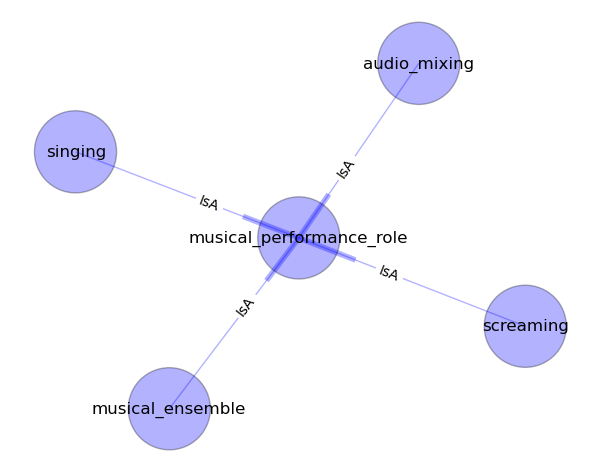
\includegraphics[height=5cm]{./images/comp_connexe_3.png}
 
   \note{Plus précisément :  16: 1, 2: 83, 3: 43, 4: 19, 5: 1, 6: 5, 9: 2, 26825: 1, 18: 1. Tout ça est très satisfaisant et RAS. L'autre ex de comp connexe bête, c'est deux éléments antonymes.}
 
\end{frame}


%%optionnel
%\begin{frame}
% \frametitle{Choix de programmation}
 
 
%\end{frame}


%%%%%%%%%%%%%%%%%%%%%%%%%%%%%%%%%%%%%
\section{TF-IDF et méthodes statistiques}
%%%%%%%%%%%%%%%%%%%%%%%%%%%%%%%%%%%%%%%

%%%%%%%%%%%%%%%%%%%%
\begin{frame}
 \frametitle{Définition de l'indice TF-IDF}
 \begin{block}{TF}
 	La fréquence d'un terme.
 \end{block}
 \begin{block}{IDF}
 	La fréquence inverse de document.\\
 	\begin{center}
 	 	$IDF_{i} =  log \frac{|D|}{|\{d_{j}: t_{i} \in d_{j}\}|}$
 	\end{center}
 \end{block}
 \begin{block}{TF-IDF}
 	\begin{center}
 		$TFIDF_{i,j} = TF_{i,j} \cdot  IDF_{i}$;
 	\end{center}
 \end{block}

 \note{Blabla}
 
 \end{frame}

%%%%%%%%%%%%%%%%%%
\begin{frame}
 \frametitle{TF-IDF pour résumer}
  \begin{block}{Poids d'une phrase}
 	La somme des valeurs TF-IDF de chaque concept dans une phrase.
 \end{block}
 \begin{itemize}
  \item Algorithme simple :
  	\begin{itemize}
  	\item Calcul les poids ;
  	\item Extraction de phrases.
  	\end{itemize}
%  \item Qualité des résumés.
 \end{itemize}

 \note{Blabla}
 
\end{frame}

%%%%%%%%%%%%%%%%%%%%%%%
\begin{frame}
 \frametitle{TF-IDF pour l'importance conceptuelle}
 \begin{itemize}
  	\item Les caractéristiques de l'importance conceptuelle
  	\begin{itemize}
  		\item Les termes importants ont une fréquence (TF) élevée~;
 		\item Les termes qui se présentent rarement dans l'ensemble du corpus ont un IDF fort.
  	\end{itemize}
  	\item Pour un résumé, le TF est calculé localement à un document, ici de manière globale.
  \end{itemize}

  \note{Blabla}
  
\end{frame}


%%%%%%%%%%%%%%%%%%%%%%%%%%%%%%%
\section{Traitement préalable des données}
%%%%%%%%%%%%%%%%%%%%%%%%%%%%%%%

%%\subsection{Analyse syntaxique}

%%%%%%%%%%%%%%%%%%%%ù
\begin{frame}
 \frametitle{Grammaires}
 Une grammaire, c'est~:
 \begin{itemize}
  \item Un ensemble de feuilles de la forme (unité syntaxique) $\rightarrow$ (liste de fonctions possibles)
  \item Un ensemble de règles pour découper la phrase en portions de plus en plus réduites.
 \end{itemize}
 
\end{frame}

%%%%%%%%%%%%%%%%%
\begin{frame}
 \frametitle{État du texte en fin d'analyse}
 Chaque mot donne~:
 \begin{itemize}
  \item lui-même, tel que présent dans le texte~;
  \item la forme normale associée~;
  \item une liste de tags catégorisant le mot (humain, idée, etc.)~;
  \item une liste de liens étiquetés vers d'autres mots de la phrase.
 \end{itemize}
 
 \note{En fin d'analyse par l'algorithme de Systran, le texte est une liste de mots contenant...}
 
\end{frame}


\begin{frame}
 \frametitle{Résolution d'anaphores}
 
 Il s'agit de remplacer les pronoms (personnels et possessifs).
 
  \begin{itemize}
   \item \textbf{Trouver} les groupes nominaux ;
   \item Pour chaque pronom, \textbf{classer} les groupes candidats par score.
  \end{itemize}

  \pause
  
  Le score dépend de :
  \begin{itemize}
   \item La position absolue (début de phrase) ;
   \item La \textbf{position relative} au pronom ;
   \item Caractéristiques grammaticales relatives au pronom ;
   \item Caractéristiques grammaticales (défini, indéfini, nom propre).
  \end{itemize}

 
 \note{Il s'agit de supprimer les ambiguités liées à l'utilisation de pronoms. Interviennent dans le score : éloignement vis-à-vis du pronom, correspondances de genre, de nombre, du caractère humain/non-humain, apparaître au début d'une phrase, GN répété, GN précédé d'une préposition ou non, GN sujet gagne en score, GN indéfini - avec article indéfini -, GN avec un nom propre gagne en score}
 
\end{frame}


\section{Traitement du réseau}

\subsection{Workspace}

\begin{frame}
  \frametitle{Workspace}

  \begin{block}{Structure}
    \begin{itemize}
      \item «~Tableau noir~» contenant les structures en cours de construction
      \item «~Projection~» du texte dans un espace plus abstrait
    \end{itemize}
  \end{block}
  \begin{block}{Intérêt}
    \begin{itemize}
      \item Représente l'état de compréhension du texte
      \item À la fin du traitement, les structures importantes du Workspace représentent l'information importante du texte.
    \end{itemize}
  \end{block}

\end{frame}

\begin{frame}
  \frametitle{Workspace}
 
  \begin{block}{Construction}
    \begin{itemize}
      \item Construit comme un graphe à partir du texte précédemment analysé
      \item Modifié par confrontation avec le réseau de concepts
    \end{itemize}
  \end{block}
 
\end{frame}

\subsection{Algorithme final}

\begin{frame}
 \frametitle{Algorithme final}

 \begin{enumerate}
  \item Construction du Workspace~;
  \item Dans le Workspace, groupement des entités;
  \item Activation des concepts associés aux éléments du Workspace~;
  \item Propagation de l'activation dans le Réseau de Concepts~;
  \item Suppression des éléments du Workspace correspondant aux concepts les moins activés.
 \end{enumerate}
 
 \note{L'algorithme de résumé en tant que tel utilise toutes les structures précédemment mentionnées.}
\end{frame}

\begin{frame}
 \frametitle{Exemples}
 
 
\end{frame}

\section{Conclusion}

\begin{frame}
 \frametitle{Conclusion}
 
C'était vraiment trop mythe comme PSC\@.
 
\end{frame}

\end{document}
